\section{Complete real-model evidence}
\label{app:real-evidence}
All displays use the completed main run. Their generators, exact inputs and full-precision table CSVs are mapped in \texttt{presentation/real-output-map.json}.

\begin{table}[htbp]
\caption{\textbf{Reporting and uncertainty choices change the observed improvement decision.} Winner 10 is selected on 256 questions from $K=4$; audit 512 estimates accuracy on 11,776 questions outside that full reservoir. First three estimates/intervals are accuracy percentages; the final row is paired winner-minus-default accuracy in percentage points. Reused CP is the ordinary nominal 95\% binomial comparator, without an exact finite-benchmark/runtime guarantee. Exact search retains the reused point estimate and uses the transformed simultaneous finite-population interval. Disjoint audit and paired gain use exact finite-population intervals. These exact intervals allocate error .025 per possible B/C design and the exported within-design multiplicity; their at-least 95\% guarantee is unconditional after runtime choice, separately per endpoint family. The first three improvement entries use the exported conservative lower-winner-above-upper-default nonoverlap rule; the paired row instead asks whether its contrast lower bound is positive. Audit-supported improvement here is not a false-positive reuse decision. Calls (s) denotes logical uncached calls for selected accuracy alone; Calls (p) denotes calls for the improvement comparison, including a differing winner/default pair on audit. Reuse/search intervals cost 1,024 for either purpose. Disjoint auditing costs 1,536 for selected accuracy alone and 2,048 for the paired comparison. The paired gain has no selected-accuracy-only entry (dash). Actual generation cost is 6,144 main answers,3,072 analyzed and 3,072 retained but excluded, plus 114 validation calls and setup/failure overhead.}
\label{tab:real-reporting}
\centering
{\fontsize{8}{9}\selectfont\begin{tabular}{lrrrrr}
\toprule
Report & Estimate & Interval & Improvement & Calls (s) & Calls (p) \\
\midrule
Reused CP & 36.72 & [30.80, 42.95] & No & 1,024 & 1,024 \\
Exact search & 36.72 & [28.55, 45.46] & No & 1,024 & 1,024 \\
Disjoint audit & 25.39 & [21.27, 29.87] & Yes & 1,536 & 2,048 \\
Paired audit gain (pp) & 8.59 & [2.88, 14.14] & Yes & --- & 2,048 \\
\bottomrule
\end{tabular}
}
\end{table}

\clearpage

\begin{table}[htbp]
\caption{\textbf{Calibration, width, selection quality and cost are distinct reporting criteria.} Entries use 20,000 iid whole-row repetitions from the known 768-row empirical distribution at the declared setting $n=256$/$K=4$. Bias is report minus that protocol's selected candidate's true cache accuracy; bias/width are percentage points, coverage/quality percentages. Parentheses are MCSEs. Simultaneous CP retains the reused point score; reuse, simultaneous and extra audit share full-search quality. The extra audit uses 256 additional question draws; question split uses 128 selection/128 report draws, and call split uses 204 selection/208 report draws. Calls are hypothetical uncached totals 1,024/1,024/1,280/640/1,024, respectively, with no new inference during resampling. They differ from the primary disjoint audit 512 and actual 6,144 generated main answers. Width/quality MCSEs and exact selection/report counts accompany the full-precision table CSV. Displayed values rounded to 0.00 do not imply zero error.}
\label{tab:real-cache-methods}
\centering
{\fontsize{8}{9}\selectfont\begin{tabular}{lrrrrr}
\toprule
Report & Bias (pp) & Coverage (\%) & Width (pp) & Quality (\%) & Calls \\
\midrule
Reused CP & 0.21 (0.020) & 95.43 (0.148) & 11.46 & 29.02 & 1,024 \\
Simultaneous CP & 0.21 (0.020) & 98.91 (0.074) & 14.46 & 29.02 & 1,024 \\
Extra audit & -0.03 (0.020) & 95.51 (0.146) & 11.43 & 29.02 & 1,280 \\
Question split & -0.03 (0.029) & 96.60 (0.128) & 16.23 & 28.75 & 640 \\
Call split & -0.01 (0.022) & 96.15 (0.136) & 12.70 & 28.94 & 1,024 \\
\bottomrule
\end{tabular}
}
\end{table}

\begin{table}[htbp]
\caption{\textbf{Paired-row bootstrap sensitivity retains substantial question-pool uncertainty.} At $K=4$ and $n=64$/256, original means are from 20,000 conditional subset-selection repetitions; percentile ranges use 1,000 outer bootstrap draws with 2,000 inner selection repetitions each. Search and audit pools are independently resampled as paired candidate vectors, rerunning selection. Both the search-minus-audit gap and selected-minus-default audit gain are in percentage points. These are approximate 95\% empirical-bootstrap sensitivity ranges without finite-population correction or an exact/conditional-on-trigger coverage guarantee; inner MC error remains at $n=64$. They do not replace the exact runtime-protected primary intervals.}
\label{tab:real-bootstrap}
\centering
{\fontsize{8}{9}\selectfont\begin{tabular}{rlrr}
\toprule
Search n & Quantity (pp) & Original mean & Bootstrap 95\% range \\
\midrule
64 & Search minus audit & 11.55 & [5.45, 18.46] \\
64 & Paired audit gain & 8.45 & [5.26, 11.65] \\
256 & Search minus audit & 11.33 & [4.69, 18.55] \\
256 & Paired audit gain & 8.59 & [5.46, 11.91] \\
\bottomrule
\end{tabular}
}
\end{table}

\clearpage

\begin{figure}[htbp]
\centering
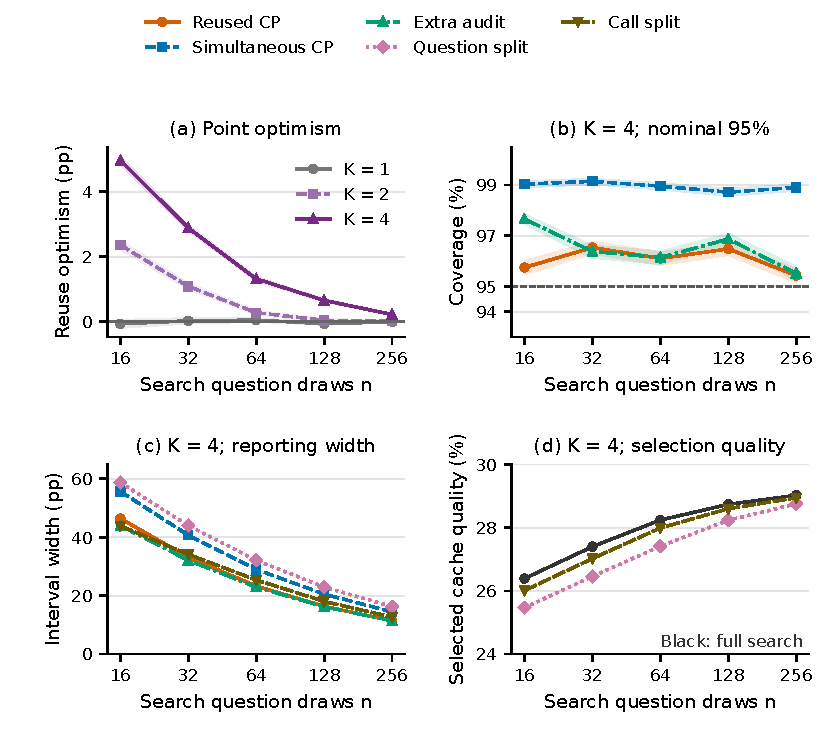
\includegraphics[width=\linewidth]{figures/real-cache.pdf}
\caption{\textbf{Positive point optimism occurs without observed nominal undercoverage in this small bank.} Conditional on the retained 768-row/four-candidate correctness cache, whole paired question rows are sampled iid with replacement, repeating full selection/reporting 20,000 times per n/K cell. The selected candidate's exact cache mean is the known target; it is distinct from remaining-benchmark accuracy. (a) Reused-score optimism for frozen-prefix K=1,2,4; adding candidates changes bank membership and true cache qualities. (b) Nominal 95\% selected-target CP coverage at $K=4$, with a dashed 95\% reference. (c) Mean interval width for all five reporting methods. (d) Selected cache quality for full search (black), equal-total-question-draw split and equal-total-call split. Reuse, simultaneous intervals and extra audit share the full-search winner. Bands are marginal 95\% Monte Carlo intervals: exact binomial intervals for coverage and mean$\pm$1.96 MCSE otherwise. They measure conditional computational error, not between-model or audit-pool uncertainty. At $K=4$, optimism declines from 4.97 pp at $n=16$ to 0.21 pp at $n=256$, while naive coverage across the entire 15-cell grid is 95.290--97.585\%. This setting does not reproduce the synthetic large-bank undercoverage. Simultaneous intervals retain the reused point estimate; the audit costs extra calls and splits can choose different candidates. The companion numerical table states budgets.}
\label{fig:real-cache-full}
\end{figure}
\clearpage
\begin{figure}[htbp]
\centering
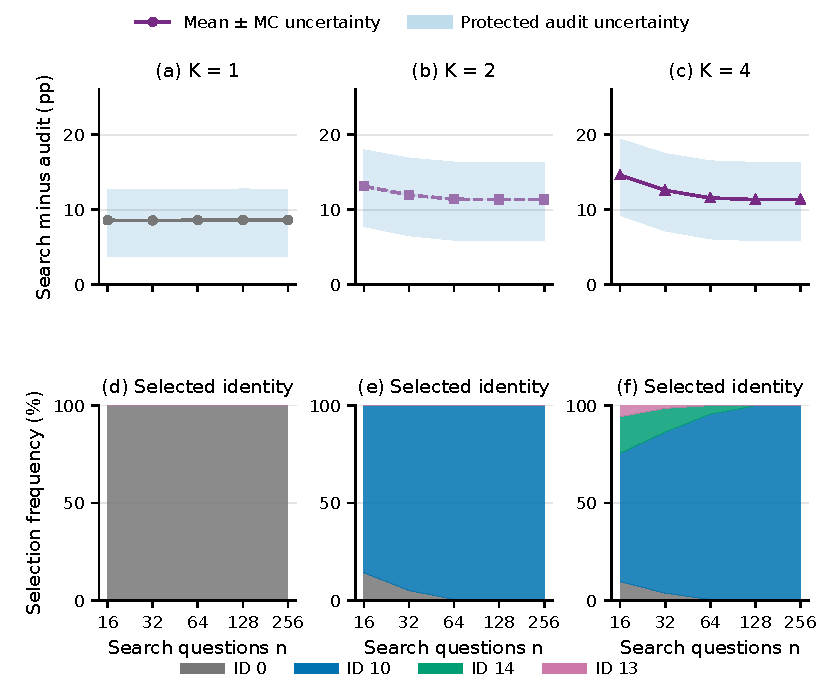
\includegraphics[width=\linewidth]{figures/real-conditional.pdf}
\caption{\textbf{The shared search--audit gap remains visible at $K=1$ and after repeated selection.} Columns use the frozen candidate-prefix sizes $K=1,2,4$; rows of the response matrix are kept paired across candidates. Top: mean selected search score minus audit score over 20,000 subset-selection repetitions at each n, conditional on one search/audit matrix. Narrow bands around curves are mean$\pm$1.96 conditional MCSE; blue regions are the analysis-exported bank-simultaneous, runtime-protected audit uncertainty bounds for the finite Monte Carlo mixture's true gap on the 11,776-item reservoir complement. These bounds retain audit uncertainty even when Monte Carlo error becomes small; they concern the finite Monte Carlo mixture rather than the infinite-repetition expectation. The displayed MC bands are marginal across cells. Each delivered endpoint family has at least 95\% unconditional protection over partition/runtime choice, with .025 error per design plus bank adjustment, and no conditional-on-trigger guarantee. Bottom: full-search winner frequencies over the same repetitions, with frozen identities labeled explicitly. All n use the complement of the entire retained 256-item search reservoir. Repetitions are computational reuse, not independent model runs or new audit datasets. Audit disagreement is not population false-superiority.}
\label{fig:real-conditional}
\end{figure}

\clearpage

\begin{figure}[htbp]
\centering
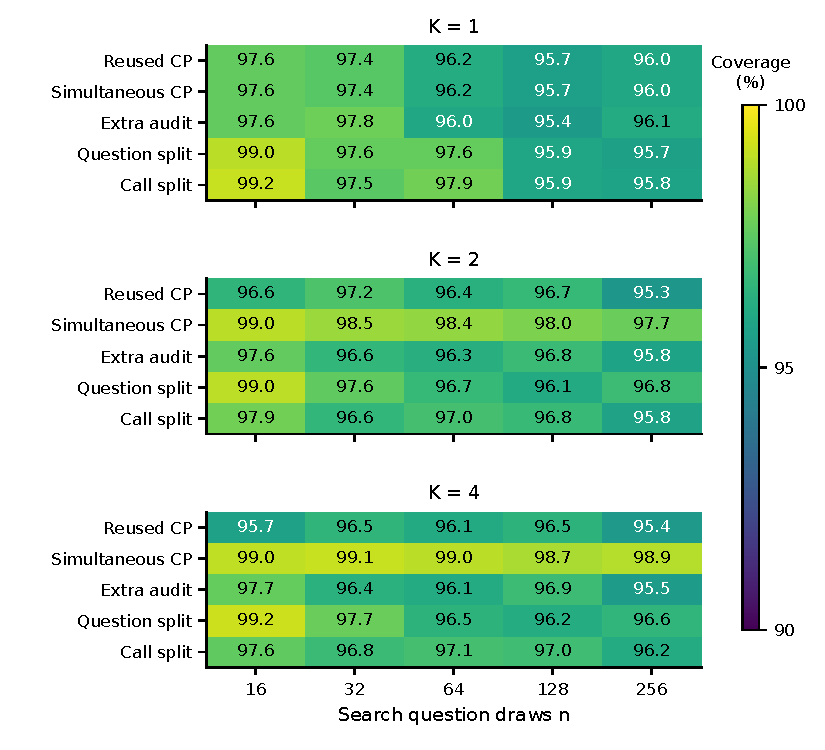
\includegraphics[width=\linewidth]{figures/real-cache-coverage-grid.pdf}
\caption{\textbf{Measured known-cache coverage remains above 95\% for naive reuse in all 15 tested cells.} Each panel fixes prefix K and displays nominal 95\% selected-target coverage for five reporting protocols across all five search sizes. Values are percentages rounded to one decimal; colors share a 90--100\% scale whose 95\% tick is the nominal reference. Each value uses 20,000 iid whole-row cache repetitions; exact 768-row empirical means supply truth. Point colors and rounded annotations omit MC intervals for space; full-precision means, MCSEs, seeds and repetition counts remain in the pinned input CSV. The main calibration figure displays marginal exact binomial MC bands, and the numerical comparison includes coverage MCSEs. Neither conservative coverage nor this small-bank null undercoverage finding establishes validity for the external audit or all prompt searches.}
\label{fig:real-cache-coverage-grid}
\end{figure}

\begin{table}[htbp]
\caption{\textbf{The conservative decision shows little false-claim activity in this cache.} Entries are event counts per 20,000 iid-cache repetitions, with reuse columns by K and the final column listing simultaneous counts for $K=1,2,4$ separately. A false event requires a selected nondefault winner's lower CP endpoint to exceed the default's upper endpoint when its exact empirical-cache quality is no better than the default. Reuse uses ordinary nominal 95\% CP endpoints; simultaneous uses .05/K marginal error. The only observed reuse event is at $n=32$/$K=4$; all simultaneous counts are zero. Zero of 20,000 still allows per-cell one-sided 95\% upper risk 0.000149775 (about 0.015\%), not zero risk or simultaneous protection across cells. The full-precision CSV includes marginal two-sided exact 95\% binomial MC intervals. This is conditional empirical-cache false-superiority, not a measured external-population error rate, paired test or claim-conditional false-discovery rate.}
\label{tab:real-cache-decisions}
\centering
{\fontsize{8}{9}\selectfont\begin{tabular}{rrrrr}
\toprule
Search n & Reuse K=1 & Reuse K=2 & Reuse K=4 & Sim K=1,2,4 \\
\midrule
16 & 0 & 0 & 0 & 0, 0, 0 \\
32 & 0 & 0 & 1 & 0, 0, 0 \\
64 & 0 & 0 & 0 & 0, 0, 0 \\
128 & 0 & 0 & 0 & 0, 0, 0 \\
256 & 0 & 0 & 0 & 0, 0, 0 \\
\bottomrule
\end{tabular}
}
\end{table}

\clearpage

\begin{figure}[htbp]
\centering
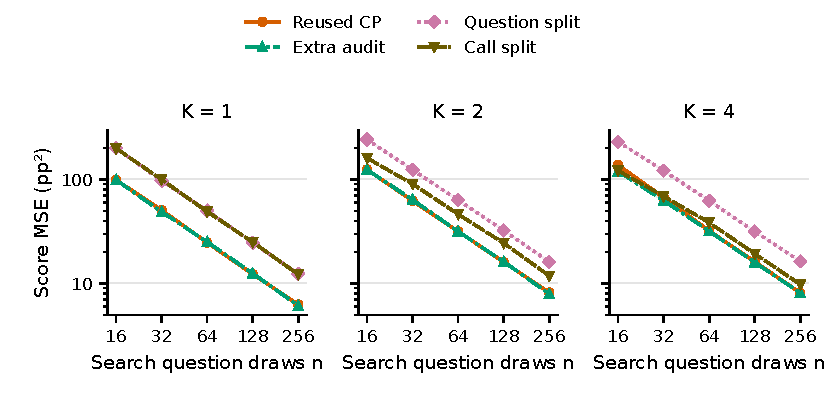
\includegraphics[width=\linewidth]{figures/real-cache-mse.pdf}
\caption{\textbf{Score error depends on reporting protocol and search size.} On the same 768-row empirical distribution, mean squared error is relative to each protocol's selected candidate's exact cache mean, in squared percentage points (log axis). Panels fix $K=1,2,4$ and retain all five n values. Bands are mean$\pm$1.96 MCSE over 20,000 iid-cache repetitions. Simultaneous CP is omitted because it preserves the reused point score and therefore has identical MSE. Extra audit uses n additional question draws/calls; question and call splits change selection sample sizes and may select different candidates. This is known-cache error, separate from squared differences against a noisy finite audit; no universal ranking or population-error claim is made.}
\label{fig:real-cache-mse}
\end{figure}

\begin{figure}[htbp]
\centering
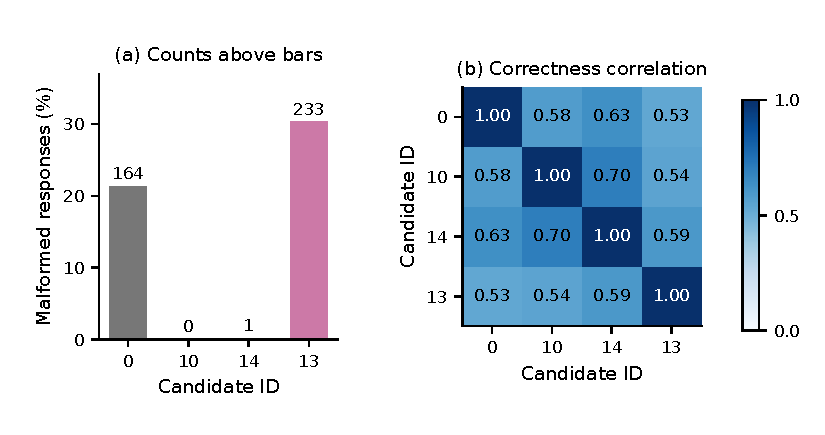
\includegraphics[width=\linewidth]{figures/real-diagnostics.pdf}
\caption{\textbf{The frozen prompt configurations differ in format adherence and share correctness patterns.} Left: malformed-output fraction for each retained candidate across 768 generated question responses; labels give counts, with a common 768 denominator. The strict frozen parser scores malformed answers wrong: default 0 has 164 malformed outputs, winner 10 none, ID 14 one and ID 13 has 233. These outcomes remain part of the tested system; no post-outcome parser repair was applied. Right: empirical correctness correlations across the same paired rows, with actual candidate IDs on both axes, a common 0--1 scale and values rounded to two decimals. These descriptive diagnostics do not establish a causal explanation of the gap or generalize across models. Full pool/category denominators and length-ending diagnostics are in the analysis package.}
\label{fig:real-diagnostics}
\end{figure}
